\section{Implement symmetrical algs in smart cards}

\subsection{Prevent information leakage}
\label{Prevent_information_leakage}

There are mainly five types of countermeasures against DPA :
\begin{itemize}
\item \textbf{\textit{Secret data masking :}}\\
\textit{boolean masking :} this method consist to Xor the secret data and with a
random number generate for each algorithm execution, mostly used to dissimulate symmetrical secret.\\
\textit{arithmetic masking :} this method consist in the application of an addition 
between random value and sensible data, mostly used to dissimulate asymmetrical secret.

\begin{itemize}
	\item[] \lokiquote{iscsc-2009-maghrebi}
\end{itemize}

\item \textbf{\textit{Dual technology :}} 
This method roughlty consists in double all the bus, while on the first bus it traveling 
a value its complement is traveling on the other bus. Overall it permit to have 
the same consumption when we are manipulating whatever the manipulated bits.

Articles about masked dual-rail pre-charged logic technology (MDPL):
\begin{itemize}
	\item[] \lokiquote{ches-2005-popp}
	\item[] \lokiquote{ches-2008-baddam}
	\item[] \lokiquote{eprint-2013-rauzy}
	\item[] \lokiquote{microj-2013-cilio}
\end{itemize}


\item \textbf{\textit{Desynchronisation :}} 
This method consist in the addition of random loop, which create random waiting.
It will be more difficult for the attacker to extract the information. 
Some like to distinguish these delay by their 
random delay: long delay -in ms-
dummy cycle: few clock cycles -in  $\mu s$-
clock jitters: short delay -in $n s$-

\item \textbf{\textit{Filter:}} This method smooth the power consumption variation. 

\begin{itemize}
	\item[] \lokiquote{sbcci-2010-legal}
\end{itemize}
	\begin{center}
		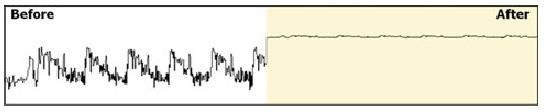
\includegraphics[width=90mm,height=25mm]{images/cri2.jpg}
	\end{center}
The previous pictures do not appear with Paul Kocher's kind authorization. 

\item \textbf{\textit{Noise :}} 
this method consist in the 'random' augmentation the consumption of chip, 
like the previous method this method makes information more difficult to extract.

\begin{itemize}
	\item[] \lokiquote{eprint-2000-hijningen}
\end{itemize}
	\begin{center}
		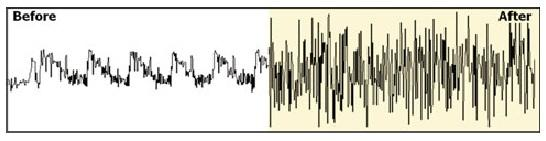
\includegraphics[width=90mm,height=25mm]{images/cri.jpg}
	\end{center}
	
\end{itemize}
All this method can be used in parallel in order to limit the power of the attacker, 
moreover those method can be used in addition of a protected implementation of the 
algorithm to be protected.
